\documentclass[prb,preprint]{revtex4-1} 
\raggedbottom
\usepackage{amsmath}
\usepackage{amsfonts}
\usepackage{graphicx}

\begin{document}

\section{Results And Analysis for Zeeman Effect}

Table \ref{energies} displays the list of current ($I$) and the associated magnetic field ($B$-field) values which were used in Fig \ref{diff} that compare line separation ($\Delta \lambda$) as it changes with the $B$-field. The $B$-field values used in Fig \ref{diff} were derived from a 6th degree polynomial fit of more extensive $I$ vs $B$-field values which are shown in Fig \ref{large}. One could potentially use a linear and square root fit in order to model the data in Fig \ref{diff} however this doesn't seem appropriate unless we have known theory which predicts such a model. As such, the polynomial fit seems more appropriate given that it can fit arbitrary data sets.

\begin{table}[h]
\caption{A table of $B$-field and line separation values as they depend on $I$}
\begin{ruledtabular}
\begin{tabular}{c c c}
$I\pm0.01$ (A) & $B\pm0.1$ (mT) & $\lambda \pm 0.4 \times10^{-6}$ (nm)\\
\hline
$3.00$& 2069.3 & 9.5\\
$4.00$& 2742.1 & 14.6\\
$5.00$& 3303.6 & 17.3\\
$6.00$& 3700.6 & 20.1\\
$7.00$& 3951.0 & 23.8\\
\end{tabular}
\end{ruledtabular}
\label{energies}
\end{table}

\begin{figure}[h]
\centering
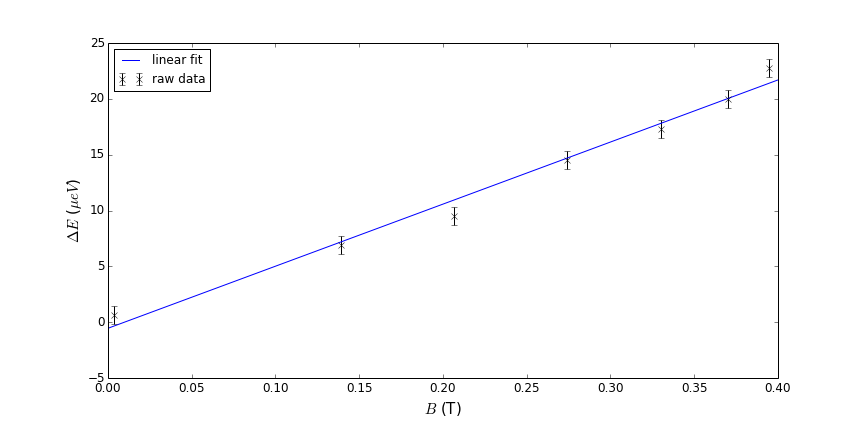
\includegraphics[width=\textwidth]{deltE_v_B.png}
\caption{The linear fit of raw $\Delta E$ measurements against extrapolated $B$ field values.}
\label{diff}
\end{figure}

\newpage

\begin{figure}[h]
\centering
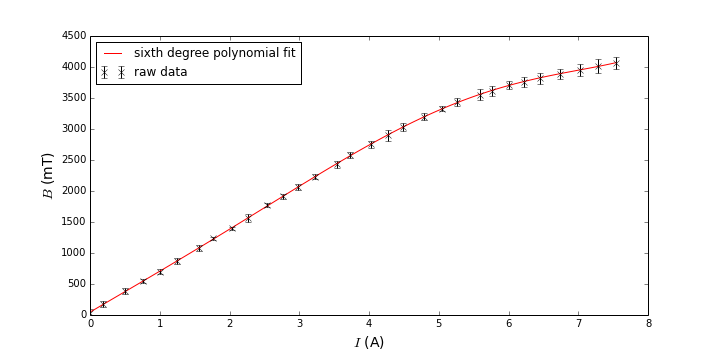
\includegraphics[width=\textwidth]{calib_IB.png}
\caption{The linear and sixth degree polynomial fits of direct $B$-field and $I$ measurements.}
\label{large}
\end{figure}

Based on the slope of the graph in Fig \ref{diff}, we find the Bohr magneton to have a value of $56\pm 3$ $\frac{\mu \text{eV}}{T}$ which agrees with the accepted value of 57.9 $\frac{\mu \text{eV}}{T}$ to within one standard deviation. The y-intercept for the linear fit was -0.5$\pm$0.8 $\mu$eV which is also in agreement with the expected value of 0.0 $\mu$eV.

\section{Conclusion}

In this report we find the Bohr magneton to have a value of $56\pm3$ $\frac{\mu \text{eV}}{T}$ which is in agreement with the accepted value. Additionally having a near zero y-intercept helps to support this measurement by confirming the expected trend.

\end{document}
